\documentclass[tikz,border=2pt]{standalone}
\usepackage{amsmath}
\usepackage{pgfplots}
\pgfplotsset{compat=1.18}
\usetikzlibrary{arrows.meta}
\begin{document}
% Matching Pennies with q = 0.4: v_1(sigma_1, sigma_2) = (2p-1)(2q-1) = 0.2 - 0.4p is linear in p,
% between v_1(T) = 1-2q = 0.2 (p = 0) and v_1(H) = 2q-1 = -0.2 (p = 1); at p = 0.7 it is -0.08.
% The maximum over p is attained at a pure strategy.
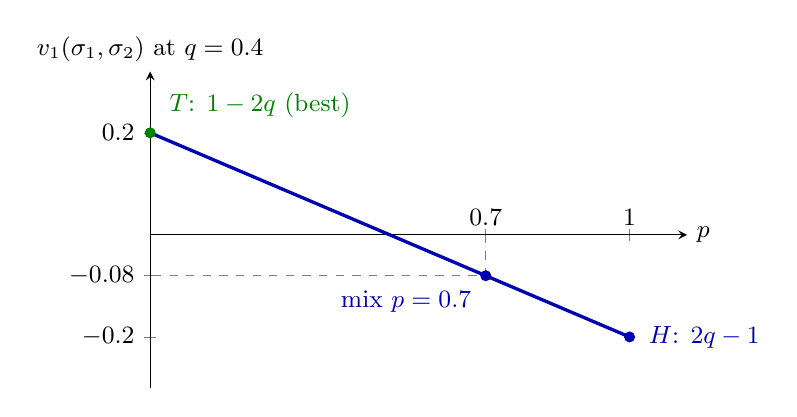
\begin{tikzpicture}[font=\small, >={Latex[length=2mm]}]
  \begin{axis}[
    axis lines=middle, xmin=0, xmax=1.12, ymin=-0.3, ymax=0.32,
    xtick={0.7,1}, ytick={-0.2,-0.08,0.2},
    yticklabels={$-0.2$,$-0.08$,$0.2$},
    xlabel={$p$}, ylabel={$v_1(\sigma_1,\sigma_2)$ at $q=0.4$},
    xlabel style={anchor=west},
    ylabel style={anchor=south},
    xticklabel style={anchor=south, yshift=2pt},
    width=8.4cm, height=5.6cm, clip=false]
    \addplot[blue!70!black, very thick, domain=0:1, samples=2] {0.2-0.4*x};
    % mixture p = 0.7
    \draw[gray, dashed, thin] (axis cs:0.7,0) -- (axis cs:0.7,-0.08) -- (axis cs:0,-0.08);
    \fill[blue!70!black] (axis cs:0.7,-0.08) circle (2pt);
    \node[blue!70!black, anchor=north east] at (axis cs:0.69,-0.09) {mix $p=0.7$};
    % pure strategies at the ends
    \fill[green!50!black] (axis cs:0,0.2) circle (2pt);
    \node[green!50!black, anchor=south west] at (axis cs:0.02,0.21) {$T$: $1-2q$ (best)};
    \fill[blue!70!black] (axis cs:1,-0.2) circle (2pt);
    \node[blue!70!black, anchor=west] at (axis cs:1.02,-0.2) {$H$: $2q-1$};
  \end{axis}
\end{tikzpicture}
\end{document}
